\section{HDASS08 Class Reference}
\label{classHDASS08}\index{HDASS08@{HDASS08}}
{\tt \#include $<$hdass08.h$>$}

Collaboration diagram for HDASS08:\begin{figure}[H]
\begin{center}
\leavevmode
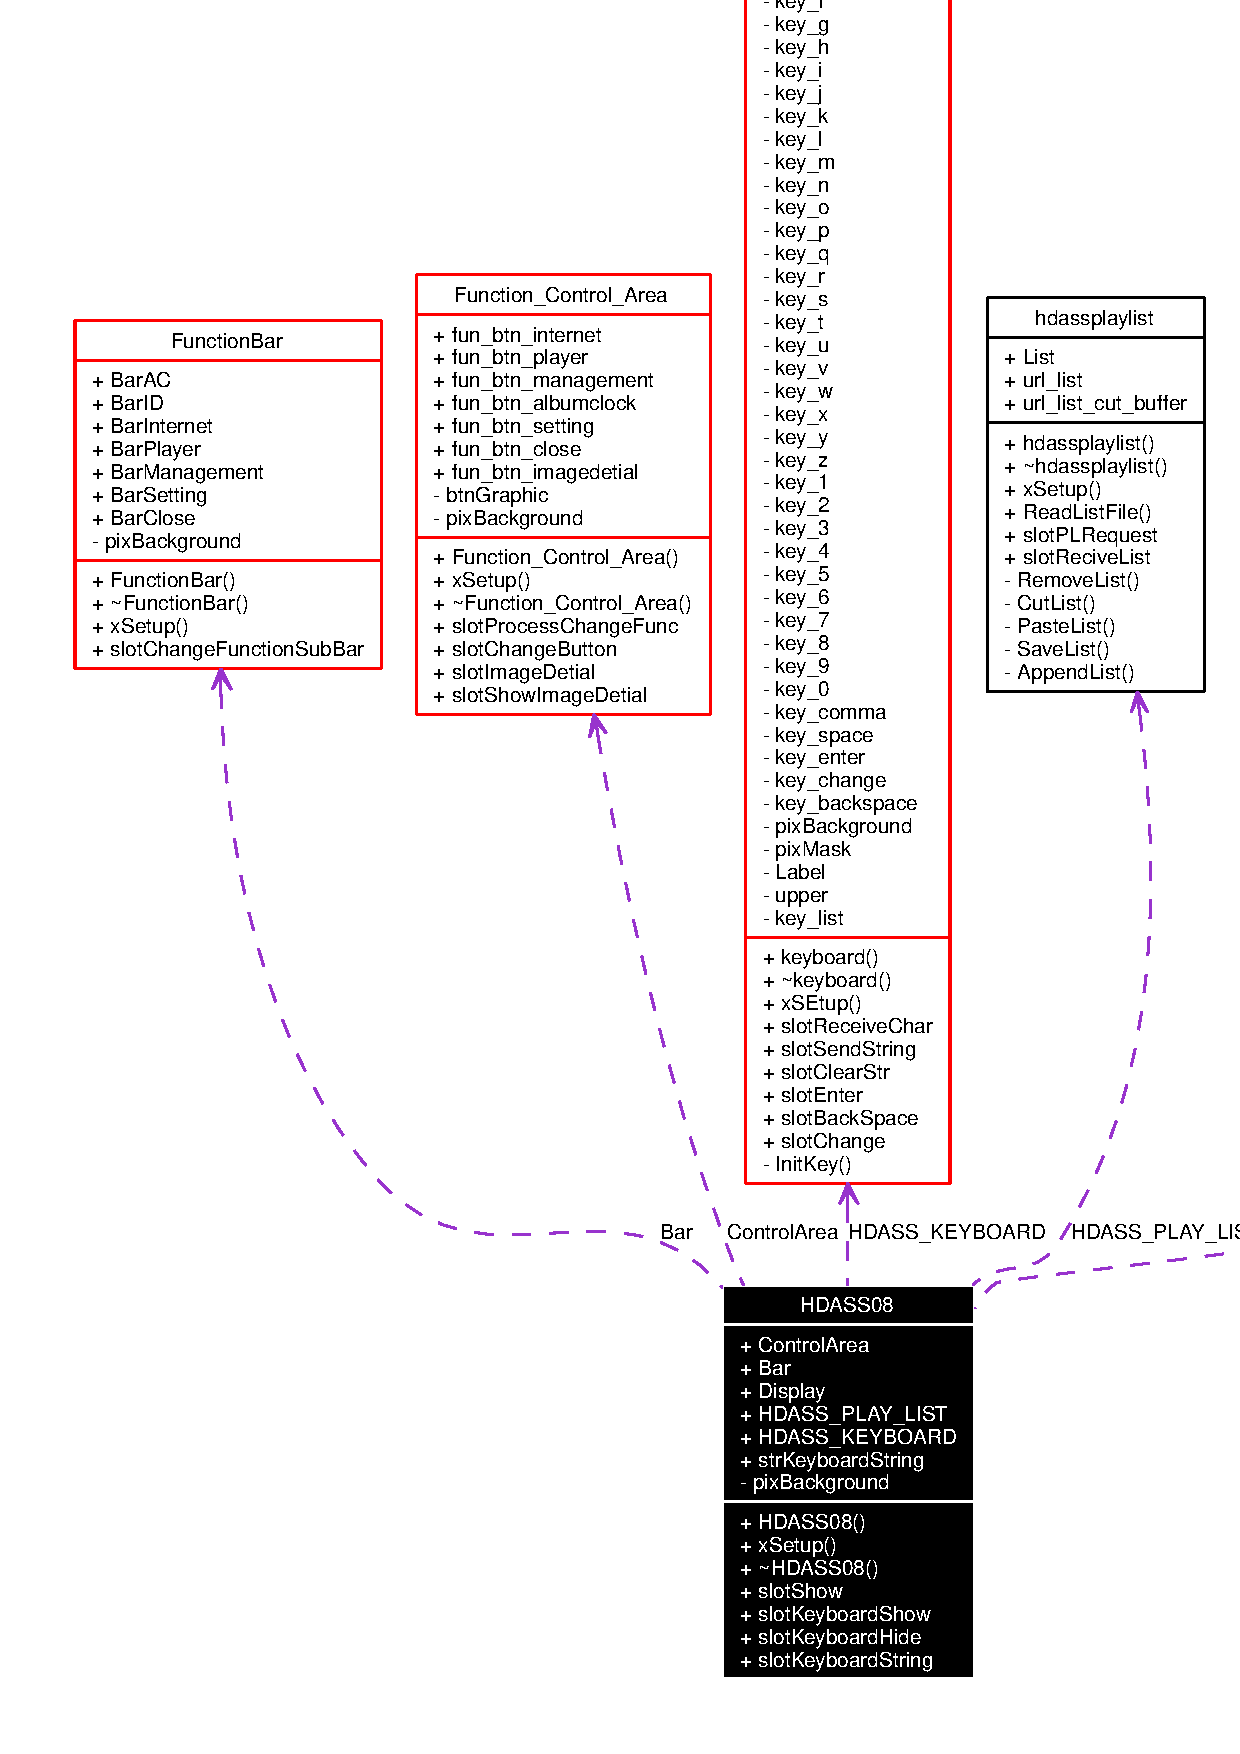
\includegraphics[width=364pt]{classHDASS08__coll__graph}
\end{center}
\end{figure}


\subsection{Detailed Description}
Application Main Window. 

\begin{Desc}
\item[Author:]sonicat $<${\tt is87098@cis.nctu.edu.tw}$>$ \end{Desc}
\begin{Desc}
\item[Version:]0.1 \end{Desc}




Definition at line 43 of file hdass08.h.\subsection*{Public Slots}
\begin{CompactItemize}
\item 
void {\bf slot\-Show} ()
\item 
void {\bf slot\-Keyboard\-Show} ()
\item 
void {\bf slot\-Keyboard\-Hide} ()
\item 
void {\bf slot\-Keyboard\-String} (QString)
\end{CompactItemize}
\subsection*{Signals}
\begin{CompactItemize}
\item 
void {\bf signal\-Mkdir} (QString)
\end{CompactItemize}
\subsection*{Public Member Functions}
\begin{CompactItemize}
\item 
{\bf HDASS08} ()
\item 
void {\bf x\-Setup} ()
\item 
virtual {\bf $\sim$HDASS08} ()
\end{CompactItemize}
\subsection*{Public Attributes}
\begin{CompactItemize}
\item 
{\bf Function\_\-Control\_\-Area} $\ast$ {\bf Control\-Area}
\item 
{\bf Function\-Bar} $\ast$ {\bf Bar}
\item 
{\bf Display\-Area} $\ast$ {\bf Display}
\item 
{\bf hdassplaylist} $\ast$ {\bf HDASS\_\-PLAY\_\-LIST}
\item 
{\bf keyboard} $\ast$ {\bf HDASS\_\-KEYBOARD}
\item 
QString {\bf str\-Keyboard\-String}
\end{CompactItemize}
\subsection*{Private Attributes}
\begin{CompactItemize}
\item 
QPixmap {\bf pix\-Background}
\end{CompactItemize}


\subsection{Constructor \& Destructor Documentation}
\index{HDASS08@{HDASS08}!HDASS08@{HDASS08}}
\index{HDASS08@{HDASS08}!HDASS08@{HDASS08}}
\subsubsection{\setlength{\rightskip}{0pt plus 5cm}HDASS08::HDASS08 ()}\label{classHDASS08_HDASS08a0}


Default Constructor 

Definition at line 29 of file hdass08.cpp.

References x\-Setup().



\footnotesize\begin{verbatim}30     : KMainWindow( 0, "HDASS08",WStyle_NoBorder | WStyle_Customize  )
31 {
32  //DAVID Setting BackGround pixmap
33   pixBackground.load("/home/sonicat/hdass08/skin-background.jpg");
34   setBackgroundPixmap(pixBackground);
35   xSetup();
36 }
\end{verbatim}\normalsize 


Here is the call graph for this function:\begin{figure}[H]
\begin{center}
\leavevmode
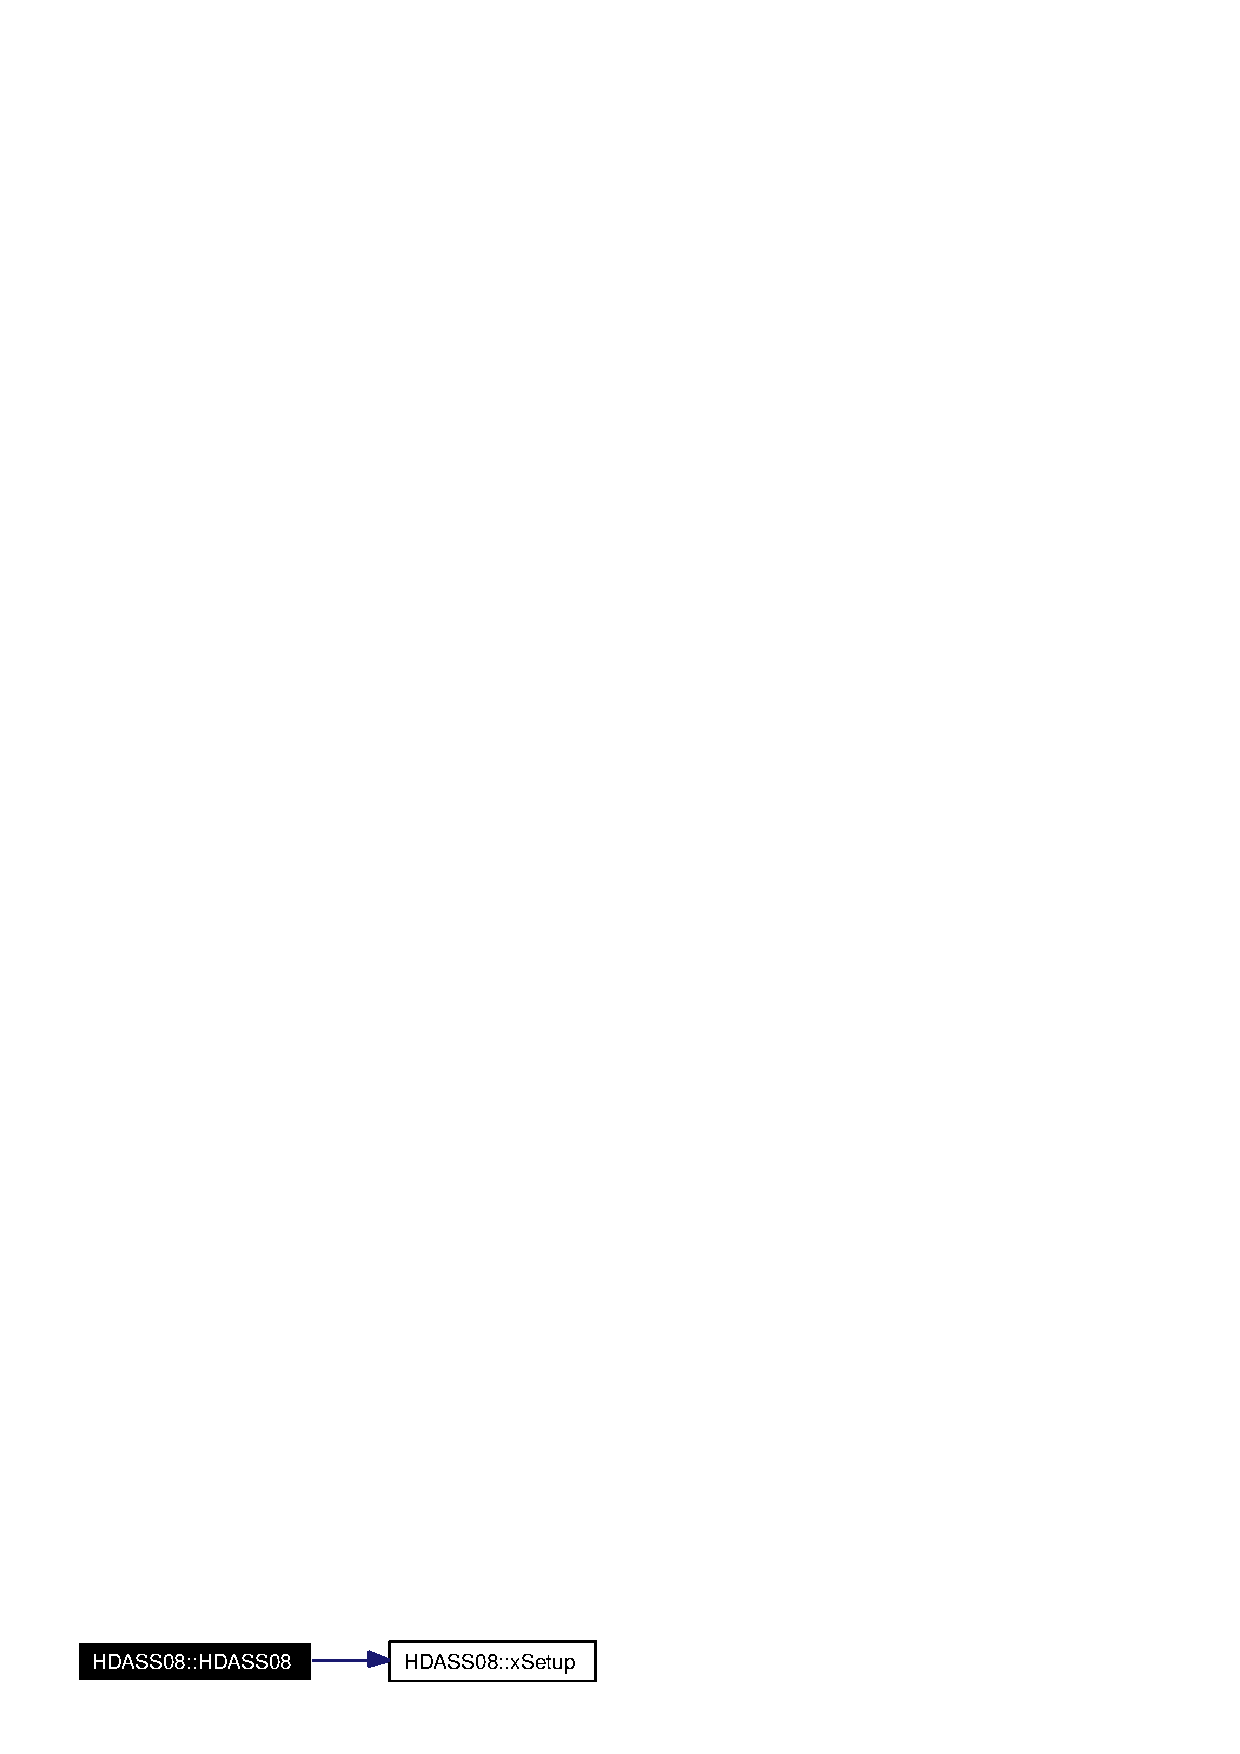
\includegraphics[width=143pt]{classHDASS08_HDASS08a0_cgraph}
\end{center}
\end{figure}
\index{HDASS08@{HDASS08}!~HDASS08@{$\sim$HDASS08}}
\index{~HDASS08@{$\sim$HDASS08}!HDASS08@{HDASS08}}
\subsubsection{\setlength{\rightskip}{0pt plus 5cm}HDASS08::$\sim${\bf HDASS08} ()\hspace{0.3cm}{\tt  [virtual]}}\label{classHDASS08_HDASS08a2}




Definition at line 38 of file hdass08.cpp.



\footnotesize\begin{verbatim}39 {
40 }
\end{verbatim}\normalsize 


\subsection{Member Function Documentation}
\index{HDASS08@{HDASS08}!signalMkdir@{signalMkdir}}
\index{signalMkdir@{signalMkdir}!HDASS08@{HDASS08}}
\subsubsection{\setlength{\rightskip}{0pt plus 5cm}void HDASS08::signal\-Mkdir (QString)\hspace{0.3cm}{\tt  [signal]}}\label{classHDASS08_HDASS08l0}




Definition at line 96 of file hdass08.moc.

Referenced by slot\-Keyboard\-Hide(), and x\-Setup().



\footnotesize\begin{verbatim}97 {
98     activate_signal( staticMetaObject()->signalOffset() + 0, t0 );
99 }
\end{verbatim}\normalsize 
\index{HDASS08@{HDASS08}!slotKeyboardHide@{slotKeyboardHide}}
\index{slotKeyboardHide@{slotKeyboardHide}!HDASS08@{HDASS08}}
\subsubsection{\setlength{\rightskip}{0pt plus 5cm}void HDASS08::slot\-Keyboard\-Hide ()\hspace{0.3cm}{\tt  [slot]}}\label{classHDASS08_HDASS08i2}




Definition at line 133 of file hdass08.cpp.

References HDASS\_\-KEYBOARD, signal\-Mkdir(), and str\-Keyboard\-String.

Referenced by x\-Setup().



\footnotesize\begin{verbatim}134 {
135   
136   HDASS_KEYBOARD->hide();
137   //Display->setEnabled(true);
138   //ControlArea->setEnabled(true);
139  // Bar->setEnabled(true);
140   emit signalMkdir(strKeyboardString);
141 }
\end{verbatim}\normalsize 
\index{HDASS08@{HDASS08}!slotKeyboardShow@{slotKeyboardShow}}
\index{slotKeyboardShow@{slotKeyboardShow}!HDASS08@{HDASS08}}
\subsubsection{\setlength{\rightskip}{0pt plus 5cm}void HDASS08::slot\-Keyboard\-Show ()\hspace{0.3cm}{\tt  [slot]}}\label{classHDASS08_HDASS08i1}




Definition at line 124 of file hdass08.cpp.

References HDASS\_\-KEYBOARD.

Referenced by x\-Setup().



\footnotesize\begin{verbatim}125 {
126    //Set Disable
127   
128    HDASS_KEYBOARD->show();
129    //Display->setEnabled(false);
130    //ControlArea->setEnabled(false);
131   // Bar->setEnabled(false);
132 }
\end{verbatim}\normalsize 
\index{HDASS08@{HDASS08}!slotKeyboardString@{slotKeyboardString}}
\index{slotKeyboardString@{slotKeyboardString}!HDASS08@{HDASS08}}
\subsubsection{\setlength{\rightskip}{0pt plus 5cm}void HDASS08::slot\-Keyboard\-String (QString)\hspace{0.3cm}{\tt  [slot]}}\label{classHDASS08_HDASS08i3}




Definition at line 142 of file hdass08.cpp.

References str\-Keyboard\-String.

Referenced by x\-Setup().



\footnotesize\begin{verbatim}143 {
144   strKeyboardString=s;
145   qWarning(strKeyboardString);
146 }
\end{verbatim}\normalsize 
\index{HDASS08@{HDASS08}!slotShow@{slotShow}}
\index{slotShow@{slotShow}!HDASS08@{HDASS08}}
\subsubsection{\setlength{\rightskip}{0pt plus 5cm}void HDASS08::slot\-Show ()\hspace{0.3cm}{\tt  [slot]}}\label{classHDASS08_HDASS08i0}




Definition at line 120 of file hdass08.cpp.



\footnotesize\begin{verbatim}121 {
122     this->show();
123 }
\end{verbatim}\normalsize 
\index{HDASS08@{HDASS08}!xSetup@{xSetup}}
\index{xSetup@{xSetup}!HDASS08@{HDASS08}}
\subsubsection{\setlength{\rightskip}{0pt plus 5cm}void HDASS08::x\-Setup ()}\label{classHDASS08_HDASS08a1}


Default Destructor 

Definition at line 42 of file hdass08.cpp.

References Display\-Area::Album, Bar, Function\-Bar::Bar\-AC, Function\-Bar::Bar\-ID, Function\-Bar::Bar\-Internet, Function\-Bar::Bar\-Management, Function\-Bar::Bar\-Player, Display\-Area::Browser, Control\-Area, Display, HDASS\_\-ACTION\_\-TYPE, HDASS\_\-KEYBOARD, HDASS\_\-PLAY\_\-LIST, Display\-Area::IA, Info\-Area::IABtn\-Volume\-Down, Info\-Area::IABtn\-Volume\-Up, mediamanagement::imgdetial, mediamanagement::img\-FIV, Sub\-Bar\-Player::m\_\-player, Display\-Area::Media, mediamanagement::music\-FIV, Info\-Area::Read\-List(), signal\-Mkdir(), slot\-Keyboard\-Hide(), slot\-Keyboard\-Show(), slot\-Keyboard\-String(), str\-Keyboard\-String, Sub\-Bar\-Internet::Sub\-Bar\-Btn\-Internet\_\-Home, Sub\-Bar\-Internet::Sub\-Bar\-Btn\-Internet\_\-Next, Sub\-Bar\-Internet::Sub\-Bar\-Btn\-Internet\_\-Previous, Sub\-Bar\-Album\-Clock::Sub\-Bar\-Btn\-Next, Sub\-Bar\-Album\-Clock::Sub\-Bar\-Btn\-Play\-NPause, and Sub\-Bar\-Album\-Clock::Sub\-Bar\-Btn\-Previous.

Referenced by HDASS08().



\footnotesize\begin{verbatim}43 {
44   //DAVID Init PlayList Here
45   HDASS_PLAY_LIST=new hdassplaylist(this,"PlayList");
46   
47   //DAVID Show the Function Control Widget 
48   
49   Display =new DisplayArea(this,"DisplayArea");
50   Display->setGeometry(0,0,800,600);
51   Display->show();
52   
53   ControlArea=new Function_Control_Area(this,"ControlArea");
54   ControlArea->setGeometry(665,465,135,135);
55   ControlArea->show();
56   
57   
58   Bar=new FunctionBar(this,"FunctionBar");
59   Bar->setGeometry(0,520,665,80);
60   Bar->show();
61   
62   HDASS_KEYBOARD =new keyboard(this,"HDASS_KEYBOARD");
63   HDASS_KEYBOARD->move(100,100);
64   HDASS_KEYBOARD->hide();
65   strKeyboardString=QString();
66   /*
67 
68   */
69   QObject::connect(ControlArea,SIGNAL(signalChangeFunc(int )),Bar,SLOT(slotChangeFunctionSubBar(int )));
70   QObject::connect(ControlArea,SIGNAL(signalBackToManagement()),Display->Media,SLOT(slotBackToManagement()));
71   QObject::connect(Bar->BarAC,SIGNAL(signalAlbumClockModeChangeToDispalyArea(int )),Display,SLOT(slotDisplayModeChange(int )));
72   QObject::connect(Bar,SIGNAL(siganlChangeDisplayAreaMode(int)),Display,SLOT(slotDisplayModeChange(int )));
73   
74   //DAVID Handle the connection between Bar and Display Buttons
75   QObject::connect(Bar->BarInternet->SubBarBtnInternet_Next, SIGNAL(clicked()), Display->Browser, SLOT(handleNext()));
76   QObject::connect(Bar->BarInternet->SubBarBtnInternet_Previous, SIGNAL(clicked()), Display->Browser, SLOT(handlePrevious()));
77   QObject::connect(Bar->BarInternet->SubBarBtnInternet_Home, SIGNAL(clicked()), Display->Browser, SLOT(handleHome()));
78   
79   //DAVID Handle the connection betwwen Album Control Buttons and all theirs corresponding function
80   QObject::connect(Bar->BarAC->SubBarBtnPrevious,SIGNAL(pressed()),Display->Album,SLOT(slotPreviousImage()));
81   QObject::connect(Bar->BarAC->SubBarBtnNext,SIGNAL(pressed()),Display->Album,SLOT(slotNextImage()));
82   QObject::connect(Bar->BarAC->SubBarBtnPlayNPause,SIGNAL(pressed()),Display->Album,SLOT(slotPlayNStop()));
83   
84   //DAVID Handle the connection between  ImageDetail Control Buttons and their  corresopnding functions 
85   QObject::connect(Bar->BarID->SubBarBtnPrevious,SIGNAL(pressed()),Display->Media->imgdetial,SLOT(slotPreviousImage()));
86   QObject::connect(Bar->BarID->SubBarBtnNext,SIGNAL(pressed()),Display->Media->imgdetial,SLOT(slotNextImage()));
87   QObject::connect(Bar->BarID->SubBarBtnPlayNPause,SIGNAL(pressed()),Display->Media->imgdetial,SLOT(slotPlayNStop()));
88   
89   //DAVID Handle the connection between Volume Buttons and the Myplayer
90   QObject::connect(Display->IA->IABtnVolumeUp, SIGNAL(pressed()), Bar->BarPlayer->m_player, SLOT(increase_volume()));
91   QObject::connect(Display->IA->IABtnVolumeDown, SIGNAL(pressed()), Bar->BarPlayer->m_player, SLOT(decrease_volume()));
92   
93   QObject::connect(Display->IA,SIGNAL(signalReadList()),HDASS_PLAY_LIST,SLOT(slotPLRequest()));
94   QObject::connect(HDASS_PLAY_LIST,SIGNAL(signalPLSend(KURL::List )),Display->IA,SLOT(slotReadListFromPlayList(KURL::List )));
95   QObject::connect(Bar->BarPlayer,SIGNAL(signalRequestPL()),HDASS_PLAY_LIST,SLOT(slotPLRequest()));
96   QObject::connect(HDASS_PLAY_LIST,SIGNAL(signalPLSend(KURL::List )),Bar->BarPlayer,SLOT(insertMedia(KURL::List )));
97   
98   QObject::connect(Display->IA,SIGNAL(signalRemoveList(KURL::List, HDASS_ACTION_TYPE )),HDASS_PLAY_LIST,SLOT(slotReciveList(KURL::List, HDASS_ACTION_TYPE )));
99   QObject::connect(Display->Media->musicFIV,SIGNAL(signalAddFileToList(KURL::List, HDASS_ACTION_TYPE )),HDASS_PLAY_LIST,SLOT(slotReciveList(KURL::List, HDASS_ACTION_TYPE )));
100   
101   QObject::connect(Bar->BarManagement,SIGNAL(signalManagementModeChange(int )),Display->Media,SLOT(slotChangeMode(int )));
102   QObject::connect(Bar->BarManagement,SIGNAL(signalMkdir()),this,SLOT(slotKeyboardShow()));
103   QObject::connect(Bar->BarManagement,SIGNAL(singalPasteFUNC_MEDIAM()),Display->Media,SLOT(slotPaste()));
104   QObject::connect(Bar->BarManagement,SIGNAL(signalCutFUNC_MEDIAM()),Display->Media,SLOT(slotCut()));
105   QObject::connect(Bar->BarManagement,SIGNAL(signalDeleteItem()),Display->Media,SLOT(slotDeleteItem()));
106   QObject::connect(Display->Media->imgFIV,SIGNAL(signalShowTheDetialofImage(KURL )),Display->Album,SLOT(slotShowFloder(KURL )));
107   
108   QObject::connect(Display->Media,SIGNAL(signalImageDetial()),ControlArea,SLOT(slotShowImageDetial()));
109   QObject::connect(Display->IA,SIGNAL(signalPlayItem(QString)),Bar->BarPlayer->m_player,SLOT(play(QString)));
110   QObject::connect(Display->IA,SIGNAL(singalPlayItem()),Bar->BarPlayer,SLOT(slotClickFromPlayList()));
111   QObject::connect(Bar->BarPlayer->m_player,SIGNAL(trackMessage(int, int, QString, QString, QString )),Display->IA,SLOT(slotHadleSongInfo(int, int, QString, QString, QString )));
112   
113   QObject::connect(HDASS_KEYBOARD,SIGNAL(signalEnter()),this,SLOT(slotKeyboardHide()));
114   QObject::connect(HDASS_KEYBOARD,SIGNAL(signalString(QString )),this,SLOT(slotKeyboardString(QString )));
115   
116   QObject::connect(Display->Media,SIGNAL(signalShowKeyboard()),this,SLOT(slotKeyboardShow()));
117   QObject::connect(this,SIGNAL(signalMkdir(QString )),Display->Media,SLOT(slotMkdir(QString )));
118   Display->IA->ReadList();
119 }
\end{verbatim}\normalsize 


\subsection{Member Data Documentation}
\index{HDASS08@{HDASS08}!Bar@{Bar}}
\index{Bar@{Bar}!HDASS08@{HDASS08}}
\subsubsection{\setlength{\rightskip}{0pt plus 5cm}{\bf Function\-Bar}$\ast$ {\bf HDASS08::Bar}}\label{classHDASS08_HDASS08o1}




Definition at line 58 of file hdass08.h.

Referenced by x\-Setup().\index{HDASS08@{HDASS08}!ControlArea@{ControlArea}}
\index{ControlArea@{ControlArea}!HDASS08@{HDASS08}}
\subsubsection{\setlength{\rightskip}{0pt plus 5cm}{\bf Function\_\-Control\_\-Area}$\ast$ {\bf HDASS08::Control\-Area}}\label{classHDASS08_HDASS08o0}




Definition at line 57 of file hdass08.h.

Referenced by x\-Setup().\index{HDASS08@{HDASS08}!Display@{Display}}
\index{Display@{Display}!HDASS08@{HDASS08}}
\subsubsection{\setlength{\rightskip}{0pt plus 5cm}{\bf Display\-Area}$\ast$ {\bf HDASS08::Display}}\label{classHDASS08_HDASS08o2}




Definition at line 60 of file hdass08.h.

Referenced by x\-Setup().\index{HDASS08@{HDASS08}!HDASS_KEYBOARD@{HDASS\_\-KEYBOARD}}
\index{HDASS_KEYBOARD@{HDASS\_\-KEYBOARD}!HDASS08@{HDASS08}}
\subsubsection{\setlength{\rightskip}{0pt plus 5cm}{\bf keyboard}$\ast$ {\bf HDASS08::HDASS\_\-KEYBOARD}}\label{classHDASS08_HDASS08o4}




Definition at line 62 of file hdass08.h.

Referenced by slot\-Keyboard\-Hide(), slot\-Keyboard\-Show(), and x\-Setup().\index{HDASS08@{HDASS08}!HDASS_PLAY_LIST@{HDASS\_\-PLAY\_\-LIST}}
\index{HDASS_PLAY_LIST@{HDASS\_\-PLAY\_\-LIST}!HDASS08@{HDASS08}}
\subsubsection{\setlength{\rightskip}{0pt plus 5cm}{\bf hdassplaylist}$\ast$ {\bf HDASS08::HDASS\_\-PLAY\_\-LIST}}\label{classHDASS08_HDASS08o3}




Definition at line 61 of file hdass08.h.

Referenced by x\-Setup().\index{HDASS08@{HDASS08}!pixBackground@{pixBackground}}
\index{pixBackground@{pixBackground}!HDASS08@{HDASS08}}
\subsubsection{\setlength{\rightskip}{0pt plus 5cm}QPixmap {\bf HDASS08::pix\-Background}\hspace{0.3cm}{\tt  [private]}}\label{classHDASS08_HDASS08r0}




Definition at line 73 of file hdass08.h.\index{HDASS08@{HDASS08}!strKeyboardString@{strKeyboardString}}
\index{strKeyboardString@{strKeyboardString}!HDASS08@{HDASS08}}
\subsubsection{\setlength{\rightskip}{0pt plus 5cm}QString {\bf HDASS08::str\-Keyboard\-String}}\label{classHDASS08_HDASS08o5}




Definition at line 63 of file hdass08.h.

Referenced by slot\-Keyboard\-Hide(), slot\-Keyboard\-String(), and x\-Setup().

The documentation for this class was generated from the following files:\begin{CompactItemize}
\item 
{\bf hdass08.h}\item 
{\bf hdass08.moc}\item 
{\bf hdass08.cpp}\end{CompactItemize}
